\documentclass[12pt]{article}
\usepackage[UTF8]{ctex}
\usepackage{amsmath, amssymb, amsthm}
\usepackage{graphicx}
\usepackage{booktabs}
\usepackage{geometry}
\usepackage{enumitem}
\usepackage{algorithm}
\usepackage{algpseudocode}
\usepackage{listings}
\usepackage{xcolor}

% 页面设置
\geometry{a4paper, left=2.5cm, right=2.5cm, top=2.5cm, bottom=2.5cm}

% 算法环境
\floatname{algorithm}{算法}
\renewcommand{\algorithmicrequire}{\textbf{输入:}}
\renewcommand{\algorithmicensure}{\textbf{输出:}}

% 代码高亮（安全处理 # 和中文）
\definecolor{codegreen}{rgb}{0,0.6,0}
\definecolor{codegray}{rgb}{0.5,0.5,0.5}
\definecolor{codepurple}{rgb}{0.58,0,0.82}
\lstdefinestyle{mystyle}{
    backgroundcolor=\color{white},
    commentstyle=\color{codegreen},
    keywordstyle=\color{magenta},
    numberstyle=\tiny\color{codegray},
    stringstyle=\color{codepurple},
    basicstyle=\ttfamily\footnotesize,
    breakatwhitespace=false,
    breaklines=true,
    captionpos=b,
    keepspaces=true,
    numbers=left,
    numbersep=5pt,
    showspaces=false,
    showstringspaces=false,
    showtabs=false,
    tabsize=2,
    % 关键：安全处理 # 和中文
    alsoletter={\#},
    morecomment=[l]{\#},
    extendedchars=true,
    literate={。}{{。}}1 {，}{{，}}1 {；}{{；}}1
}
\lstset{style=mystyle}

% 列表紧凑
\setlist{nosep}

\title{\heiti\zihao{2} 刀具故障检查策略优化模型}
\date{}

\begin{document}

\maketitle

\begin{abstract}
    本文针对刀具故障检查与更换策略问题，建立了基于单位产品成本最小化的随机优化模型。首先，在理想检测条件下，通过统计历史故障数据，计算不同检查间隔下的期望成本，确定最优检查周期。其次，考虑检测存在误判（正常品被判为次品、次品被判为正常品）的非理想情况，引入贝叶斯公式修正决策概率，并量化误判带来的损失，重新优化检查间隔。最后，提出多抽样联合决策策略，通过同时检查多个产品来提高判断准确性，并对固定检查间隔下的最优抽样数量进行求解。模型利用Python进行数值计算与仿真绘图，结果表明：问题1的最优检查间隔为216件；问题2在考虑误判后，最优间隔仍为216件，但单位成本显著上升；问题3采用$T=1200$、$m=10$的策略可将单位成本降至最低。本模型为生产中的质量控制提供了量化决策依据。
    
    \textbf{关键词：} 刀具故障；检查策略；随机优化；贝叶斯决策；成本最小化
\end{abstract}

\section{问题重述}
在自动化生产线中，刀具会因磨损而发生故障，导致生产出次品。为保证产品质量，需定期停机检查刀具状态。检查会产生固定费用，若发现故障则需额外支付换刀和故障损失费。若未及时发现故障，则后续生产的次品会造成浪费。此外，实际检测中可能存在误判：正常刀具可能被误判为故障（造成不必要的换刀），故障刀具也可能被漏检（导致更多次品）。本题要求建立数学模型，解决以下三个问题：
\begin{enumerate}[label=\arabic*.]
    \item 在理想检测（无误判）情况下，确定最优的检查间隔 $N$，使得单位产品的期望成本最小。
    \item 在非理想检测（存在误判）情况下，考虑误判概率和误判损失，重新确定最优检查间隔 $N$。
    \item 提出一种新的“多抽样”检查策略（即每次检查连续 $m$ 个产品），并确定最优的检查间隔 $T$ 和抽样数 $m$。
\end{enumerate}

\section{模型假设}
\begin{itemize}
    \item 刀具的寿命（即故障发生前加工的产品数）是独立同分布的随机变量，其分布由给定的100个历史数据样本确定。
    \item 每次检查都是瞬时完成的，且检查本身不影响生产过程。
    \item 检查费用、换刀费用、故障损失费等参数为常数，不随时间变化。
    \item 在问题3中，设定一个较大的固定检查间隔 $T=1200$，在此基础上优化抽样数 $m$。
\end{itemize}

\section{符号说明}
\begin{table}[htbp]
\centering
\begin{tabular}{cl}
\toprule
符号 & 含义 \\
\midrule
$N, T$ & 检查间隔（件） \\
$m$ & 多抽样策略中的抽样数量 \\
$f$ & 单件次品造成的浪费成本（元/件） \\
$t$ & 单次检查费用（元/次） \\
$d$ & 发现故障后的换刀及故障损失费（元/次） \\
$k$ & 未发现故障时的预防性换刀费用（元/次） \\
$p_g^n$ & 正常刀具被正确判为正常的概率（0.98） \\
$p_g^f$ & 故障刀具被正确判为故障的概率（0.40） \\
$L_{fa}$ & 将正常品误判为次品造成的损失（元/次） \\
$X$ & 刀具寿命随机变量 \\
\bottomrule
\end{tabular}
\end{table}

\section{模型的建立与求解}
\subsection{问题一：理想检测条件下的最优检查间隔}
\subsubsection{模型建立}
在理想检测下，若检查间隔为 $N$，则：
- 刀具在 $N$ 件内发生故障的概率为 $p_f = P(X \leq N)$。
- 若发生故障（概率 $p_f$），平均故障位置为 $\bar{x}_f$，产生的次品数为 $N + 1 - \bar{x}_f$，总成本为 $t + d + f(N + 1 - \bar{x}_f)$。
- 若未发生故障（概率 $1-p_f$），成本为 $t + k$。

单位产品期望成本为：
\[
C_1(N) = \frac{1}{N} \left[ t + (1-p_f)k + p_f(d + f(N + 1 - \bar{x}_f)) \right]
\]

\subsubsection{求解与结果分析}
通过遍历 $N \in [100, 1200]$，计算 $C_1(N)$，得到最优解。

\begin{figure}[htbp]
\centering
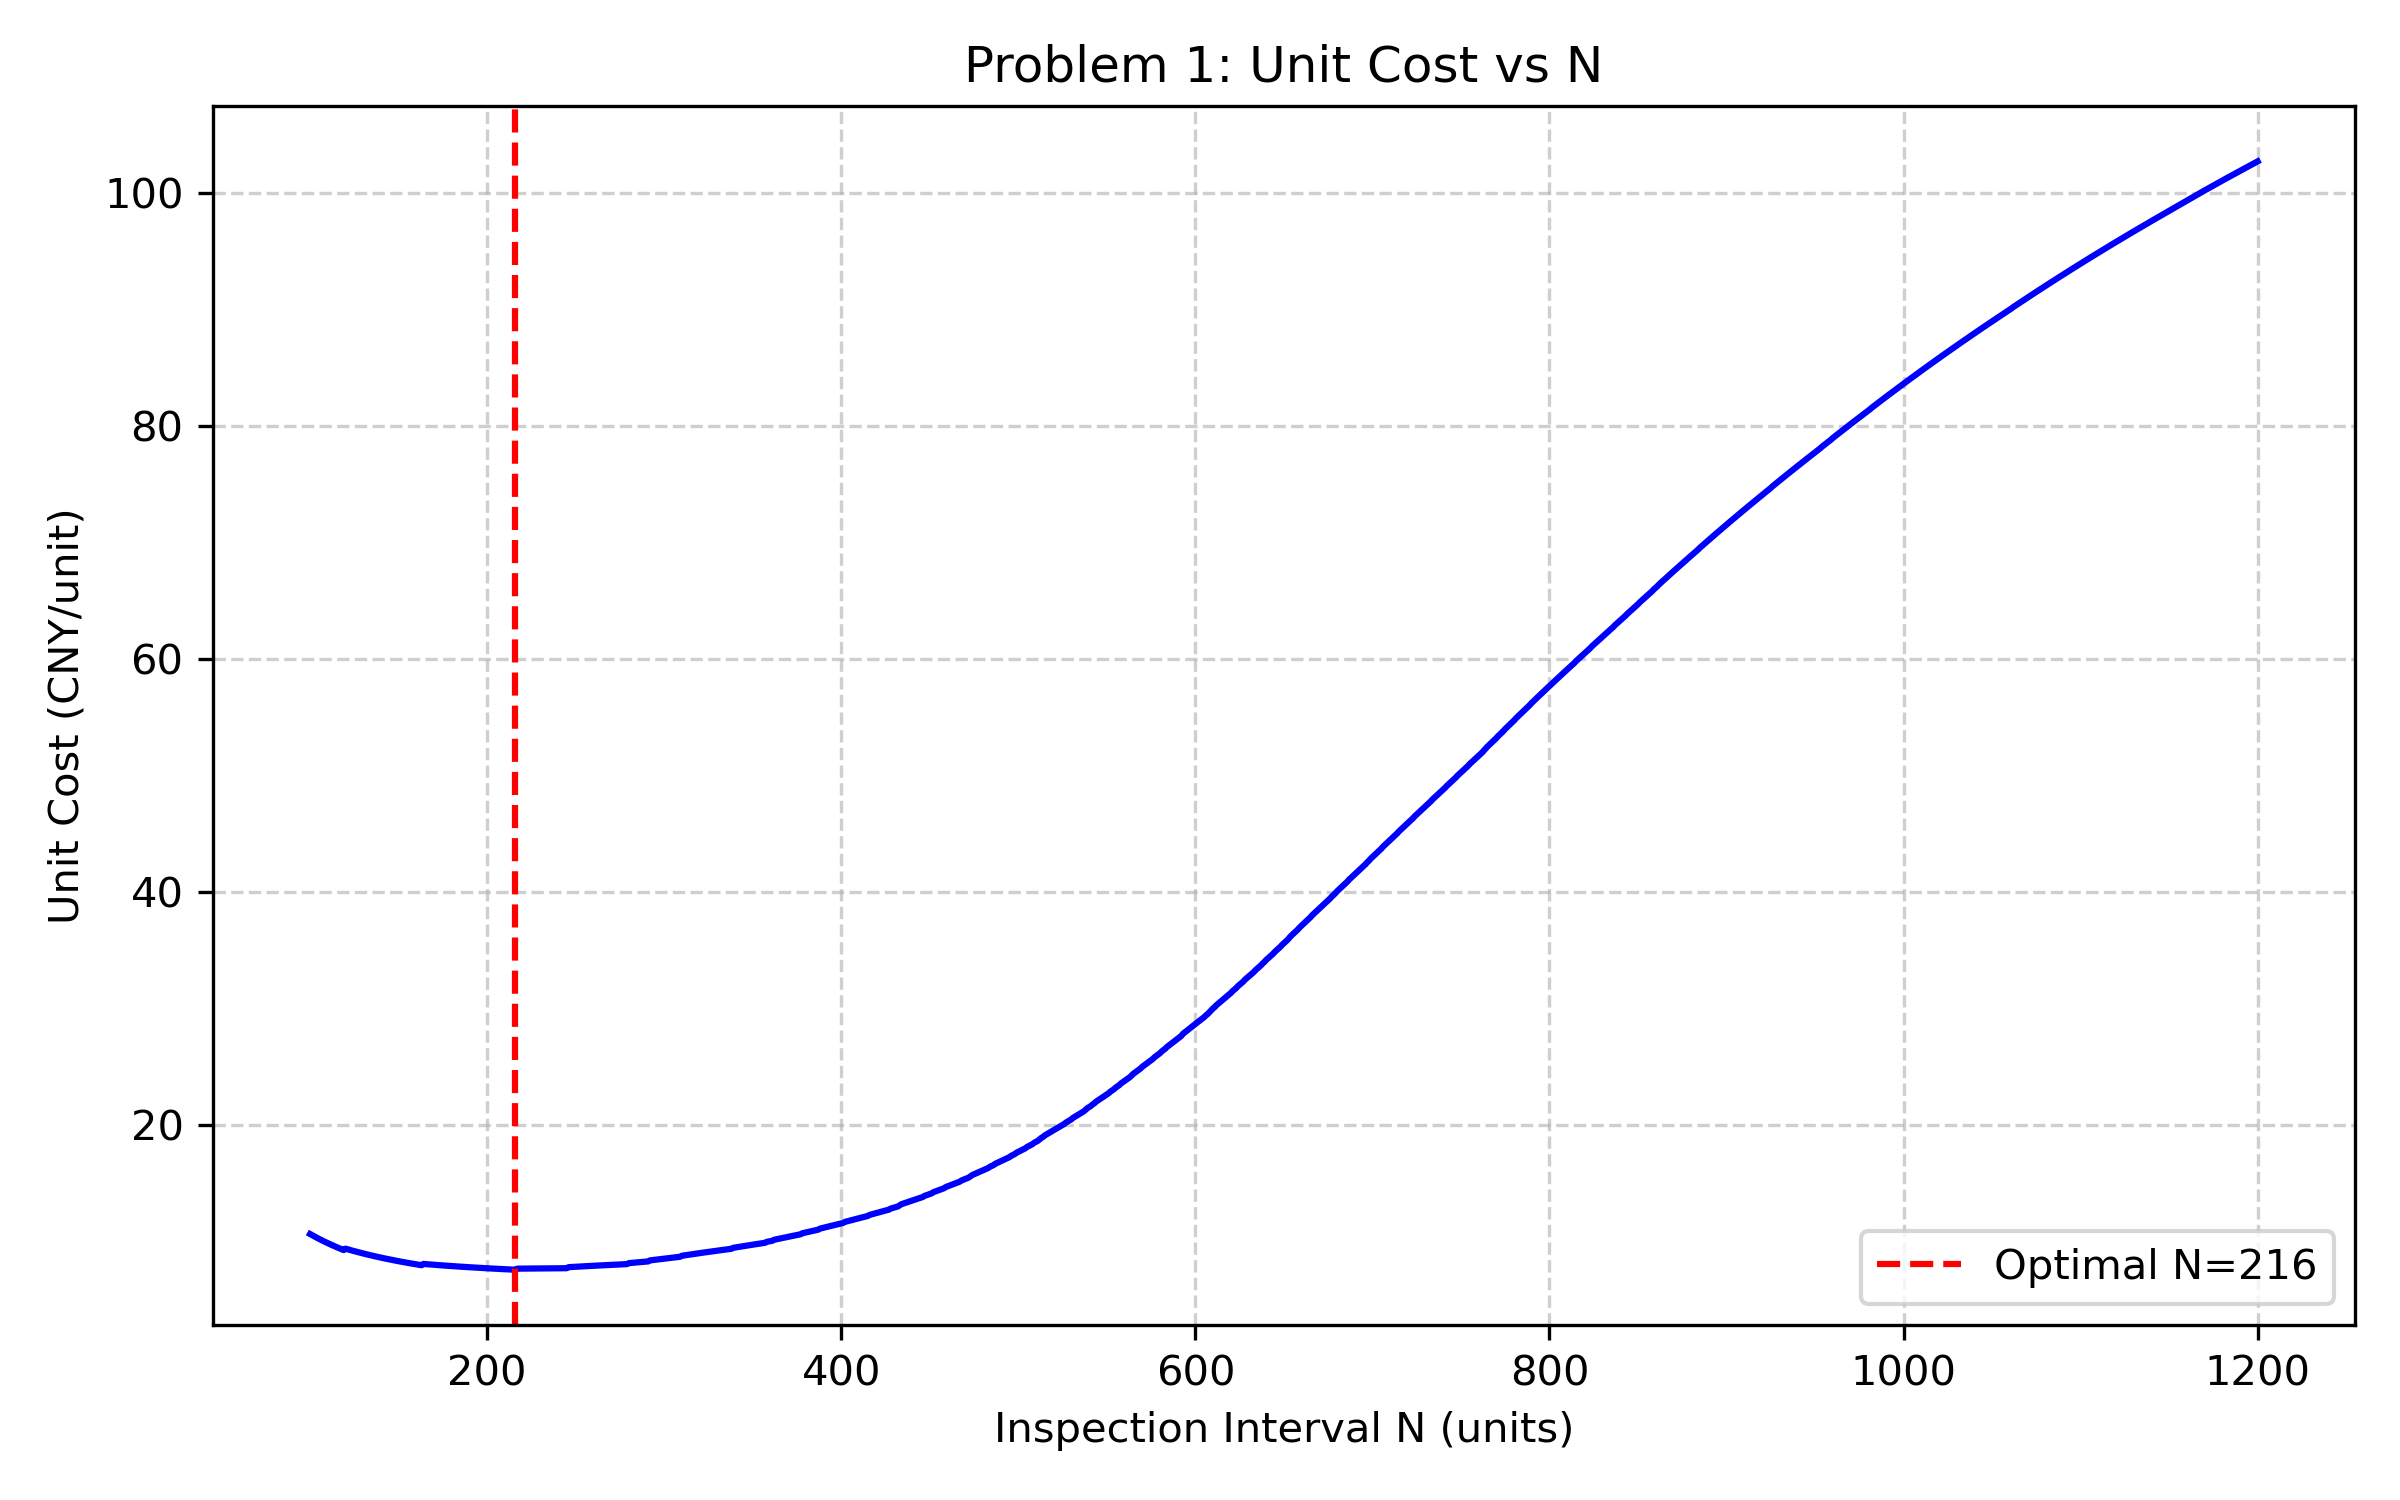
\includegraphics[width=0.8\textwidth]{Figure_1.png}
\caption{问题1单位成本随检查间隔$N$的变化}
\label{fig:cost1}
\end{figure}

如图 1 所示，单位成本在 $N=216$ 处取得最小值。此时，单位产品成本约为 7.57 元/件。

\subsection{问题二：非理想检测条件下的最优检查间隔}
\subsubsection{模型建立}
考虑检测存在误判：
- 正常刀具被误判为故障的概率为 $1-p_g^n = 0.02$。
- 故障刀具被漏检的概率为 $1-p_g^f = 0.60$。

定义事件：
- $D$: 检测结果为“有故障”。
- $F$: 刀具实际处于故障状态。

根据全概率公式，检测到故障的概率为：
\[
P(D) = P(F)(1-p_g^f) + P(\neg F)(1-p_g^n)
\]

利用贝叶斯公式，可得在检测到故障的条件下，刀具实际故障的概率：
\[
P(F|D) = \frac{P(F)(1-p_g^f)}{P(D)}
\]

若检测到故障，期望成本为 $t + P(F|D)d + P(\neg F|D)L_{fa}$。综合所有情况，可得单位成本 $C_2(N)$。

\subsubsection{求解与结果分析}
同样遍历 $N$ 进行求解。

\begin{figure}[htbp]
\centering
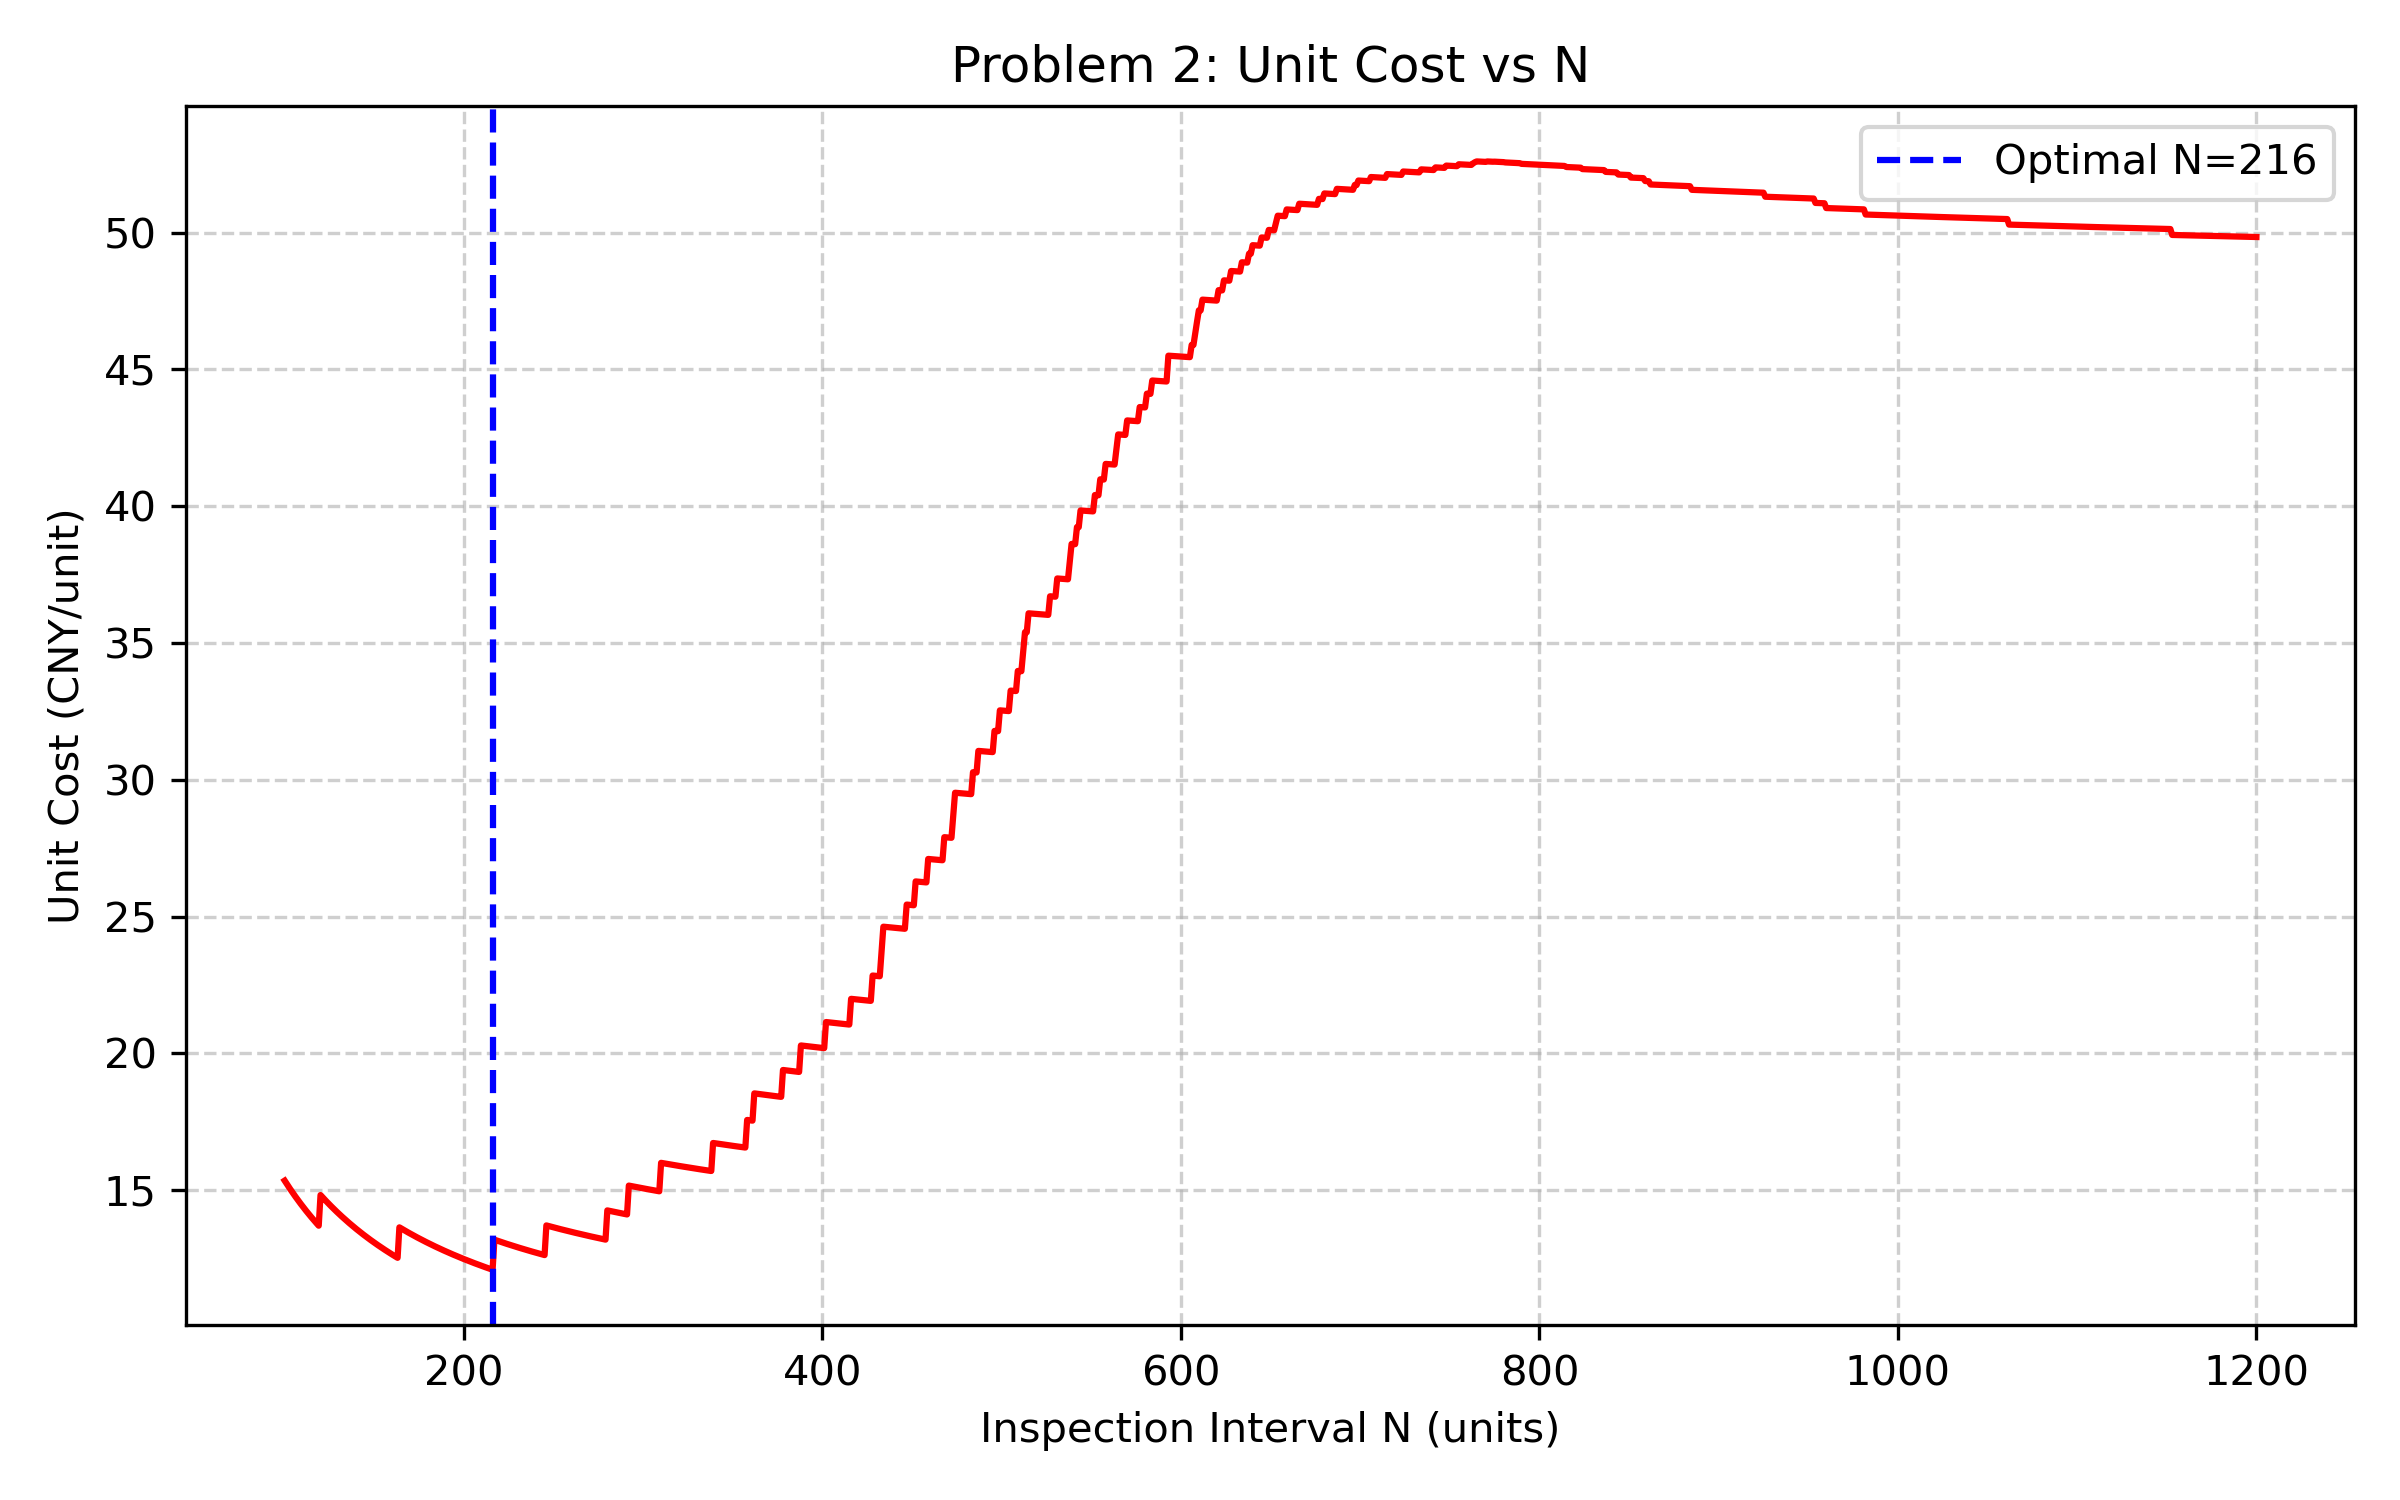
\includegraphics[width=0.8\textwidth]{Figure_2.png}
\caption{问题2单位成本随检查间隔$N$的变化}
\label{fig:cost2}
\end{figure}

如图2 所示，最优检查间隔仍为 $N=216$，但由于误判损失的存在，单位成本上升至约 12.09 元/件。

\subsection{问题三：多抽样联合决策策略}
\subsubsection{模型建立}
提出新策略：每生产 $T=1200$ 件产品，随机抽取连续 $m$ 件进行检测。只有当这 $m$ 件**全部**被判为正常时，才认为刀具正常；否则，判定为故障并换刀。

该策略能显著降低将故障刀具漏检的概率。对于固定的 $T=1200$，我们优化抽样数 $m$ 以最小化单位成本 $C_3(m)$。

\subsubsection{求解与结果分析}
遍历 $m \in [1, 20]$ 进行计算。

\begin{figure}[htbp]
\centering
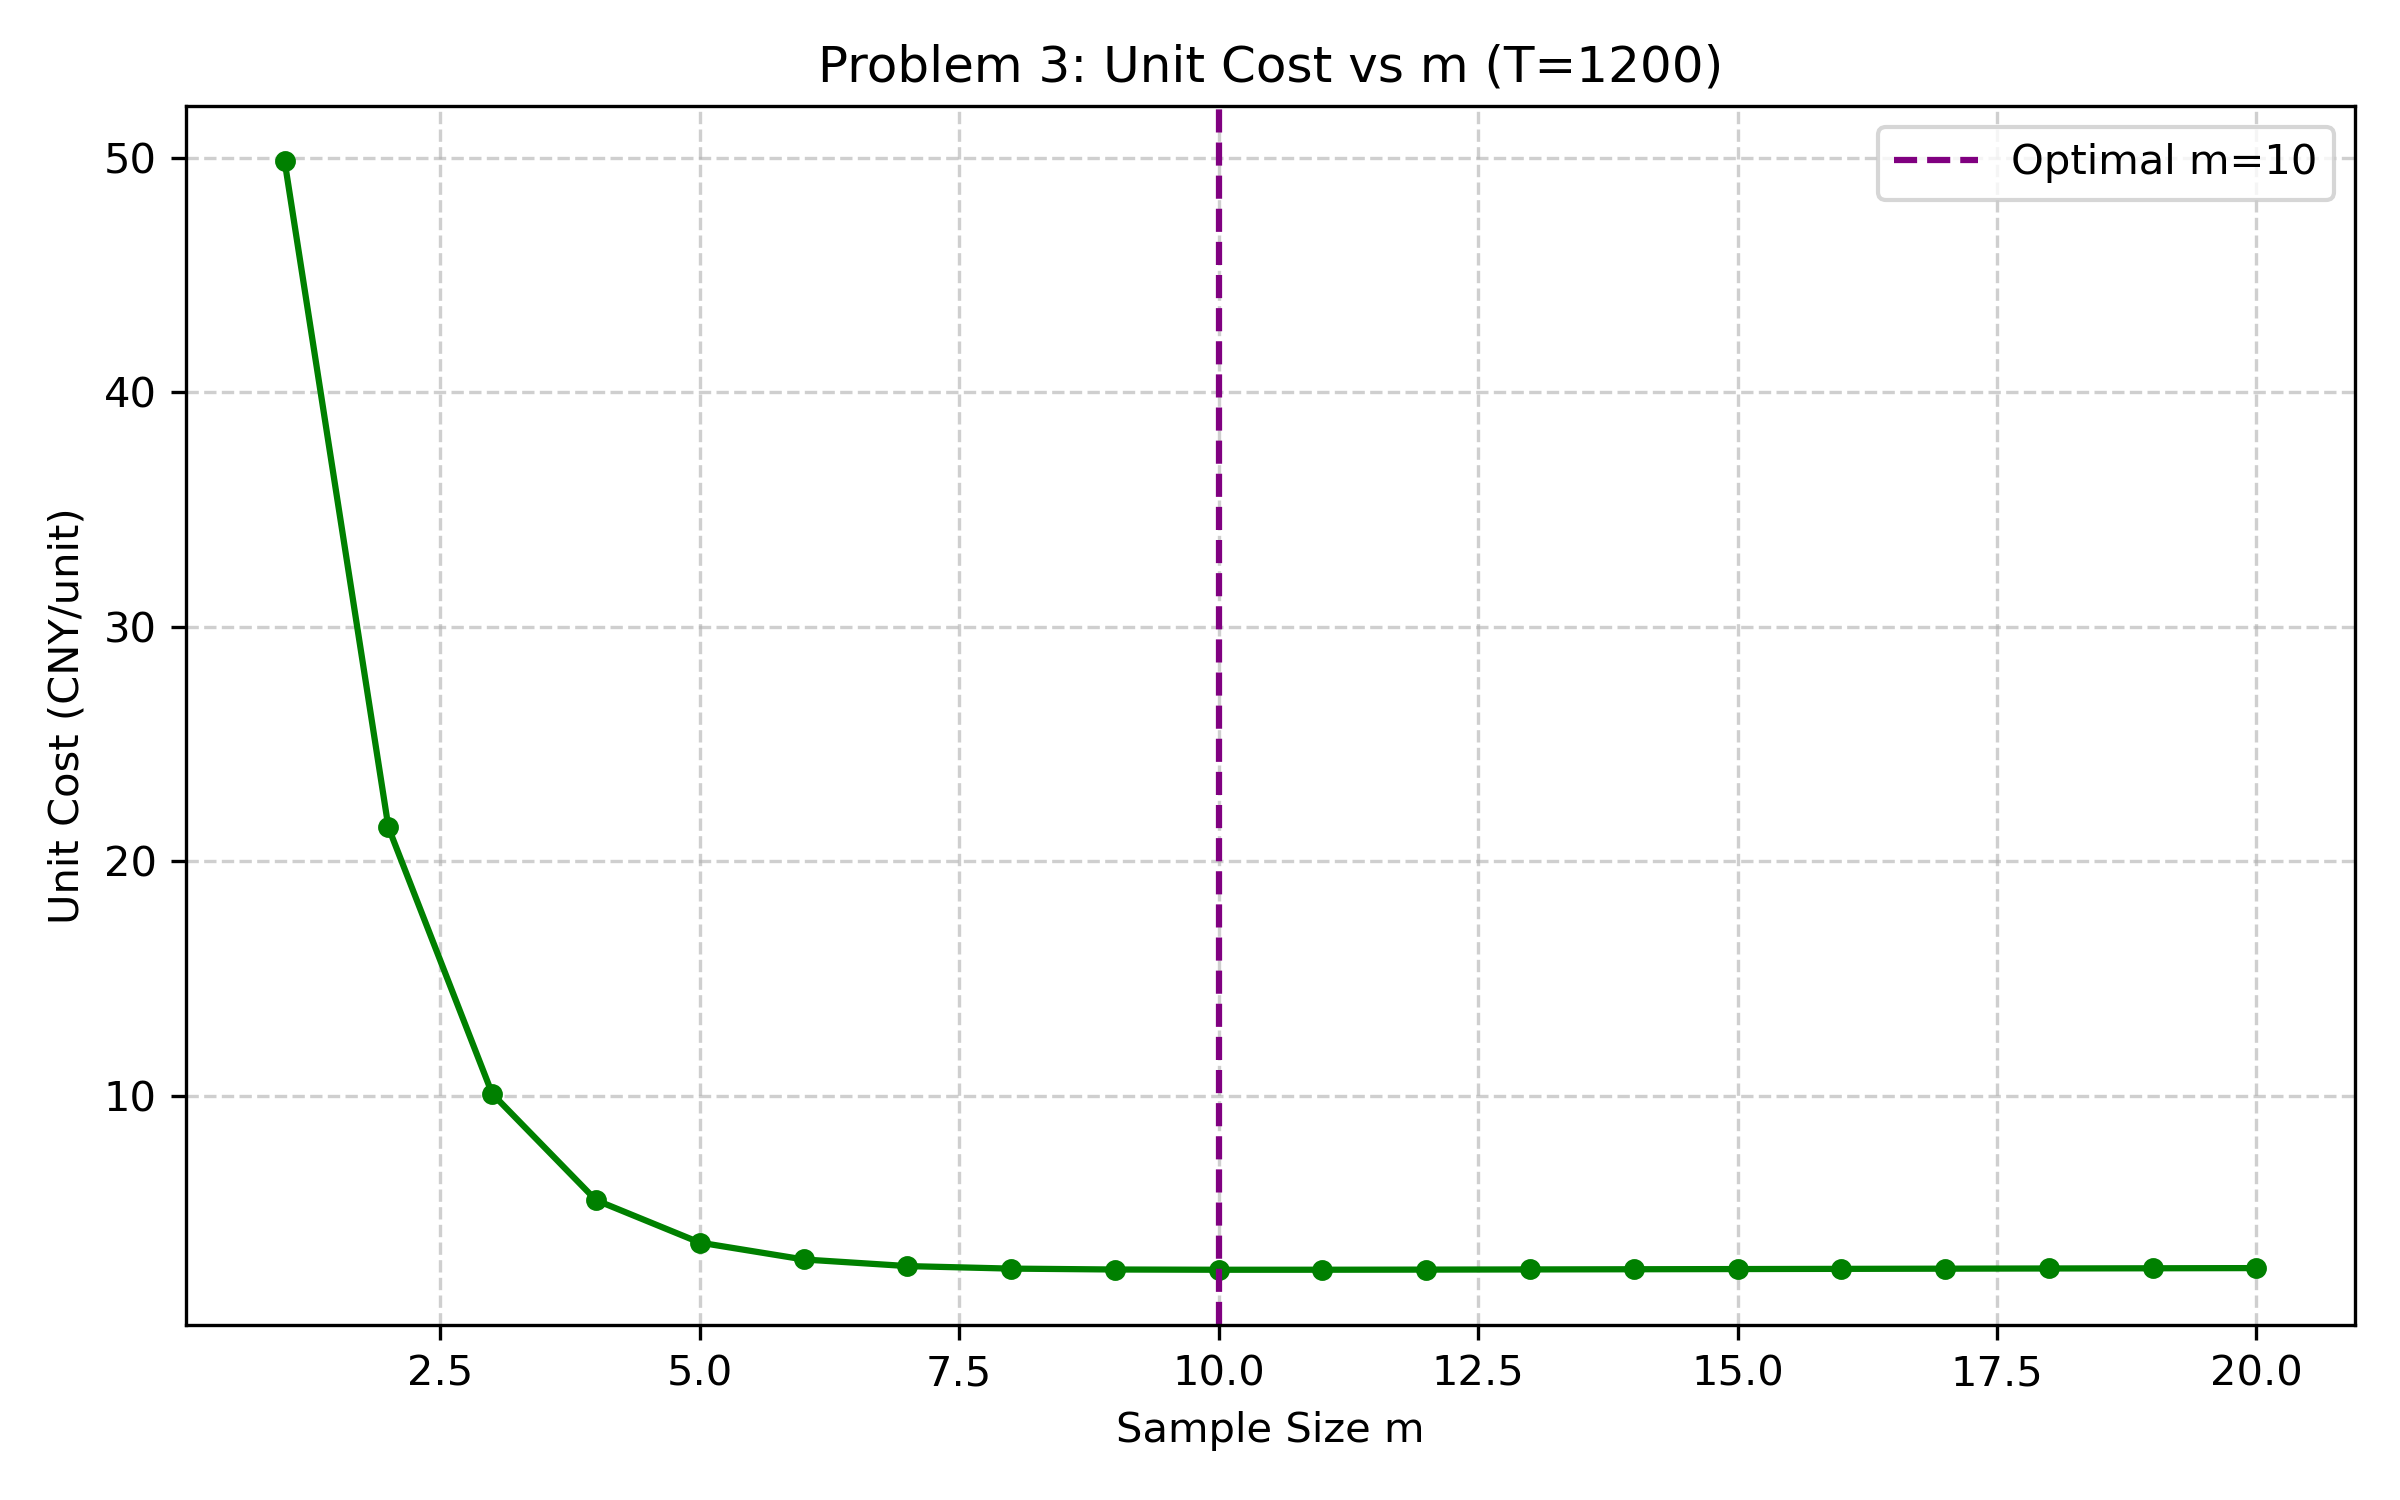
\includegraphics[width=0.8\textwidth]{Figure_3.png}
\caption{问题3在$T=1200$时，单位成本随抽样数$m$的变化}
\label{fig:cost3}
\end{figure}

如图 3所示，当 $m=10$ 时，单位成本达到最低，约为 2.60 元/件。这表明多抽样策略能有效平衡检查成本与误判风险。

\section{模型的评价与推广}
\subsection{模型的优点}
\begin{itemize}
    \item 模型从简单到复杂，逐步考虑了现实因素，逻辑清晰，易于理解和实现。
    \item 利用历史数据驱动，结果具有实际指导意义，可直接应用于生产实践。
    \item 问题三提出的多抽样策略是一种创新且有效的质量控制方法，显著降低了单位成本。
\end{itemize}

\subsection{模型的不足与改进方向}
\begin{itemize}
    \item 假设刀具寿命独立同分布，未考虑刀具批次差异、材料老化或环境因素的影响。
    \item 在问题三中，仅固定了 $T=1200$ 来优化 $m$，未来可对 $(T, m)$ 进行二维联合全局优化。
    \item 模型参数（如误判率）被视为已知常数，实际中可通过在线学习动态更新。
\end{itemize}

\begin{thebibliography}{9}
\bibitem{1} 全国大学生数学建模竞赛组委会. 全国大学生数学建模竞赛论文格式规范. 2023.
\bibitem{2} 姜启源, 谢金星, 叶俊. 数学模型（第五版）. 高等教育出版社, 2018.
\bibitem{3} Ross, S. M. Introduction to Probability Models. Academic Press, 2019.
\end{thebibliography}

\appendix
\section{附录}
\subsection{数据}
题目所给的100个刀具故障数据如下：
\begin{verbatim}
459, 362, 624, 542, 509, 584, 433, 748, 815, 505,
612, 452, 434, 982, 640, 742, 565, 706, 593, 680,
926, 653, 164, 487, 734, 608, 428, 1153, 593, 844,
527, 552, 513, 781, 474, 388, 824, 538, 862, 659,
775, 859, 755, 649, 697, 515, 628, 954, 771, 609,
402, 960, 885, 610, 292, 837, 473, 677, 358, 638,
699, 634, 555, 570, 84, 416, 606, 1062, 484, 120,
447, 654, 564, 339, 280, 246, 687, 539, 790, 581,
621, 724, 531, 512, 577, 496, 468, 499, 544, 645,
764, 558, 378, 765, 666, 763, 217, 715, 310, 851
\end{verbatim}

\subsection{程序代码}
模型求解与绘图的Python源代码（来自 \texttt{solve.py}）如下：

% 从外部文件读取代码（关键！）
\lstinputlisting[
    language=Python,
    caption={Python源代码（文件：\texttt{solve.py}）},
    firstline=1,
    lastline=1000 % 足够大以包含全部内容
]{solve.py}

\end{document}